\documentclass[aspectratio=1610]{beamer}
\usepackage{graphicx}
\usepackage{amsmath}
\usepackage{amsfonts}
\usepackage{tikz}
\usepackage{tcolorbox}
% BibLaTeX setup
\usepackage[backend=biber,style=authoryear-comp,sorting=nyt]{biblatex}
\addbibresource{refere.bib}
\usepackage[absolute,overlay]{textpos}
\usecolortheme{default}

\title{Validation of Coupled Atmospheric-Aeroelastic Model System for Wind Turbine Load Calculations for Enercon turbine}
\vspace{10mm}
\author{Aravind Venkatachalapathy}
\institute{Enercon}
\date{\today}

\begin{document}

% Slide 1: Title Slide
\frame{\titlepage}

% Slide 2: Introduction and Motivation
\begin{frame}{Introduction and Motivation}
    \begin{columns}
        \begin{column}{0.6\textwidth}
            \textbf{Research Objective:}
            \begin{itemize}
                \item Validate coupled atmospheric- aeroelastic models for accurate wind turbine simulations with Focus on Enercon turbine.
            \end{itemize}
            \vspace{5mm}
            \textbf{Traditional Aeroelastic Simulation Limitations:}\\
             \textcolor{red}{Synthetic turbulence (Kaimal/Mann spectrum) models} :
                \begin{itemize}
                    \item Assume statistically stationary, homogeneous turbulence
                    \item Pre-calculated wind fields with simplified atmospheric conditions
                    \item Limited representation of complex flow phenomena (gusts, shear, atmospheric stability)
                \end{itemize}
        \end{column}
        \begin{column}{0.4\textwidth}
                \textcolor{red}{Wake modeling deficiencies:}
                \begin{itemize}
                    \item Simplified wake models (Jensen, Frandsen) lack temporal dynamics
                    \item No feedback between turbine operation and atmospheric flow
                \end{itemize}
            
            \vfill
            \begin{center}
              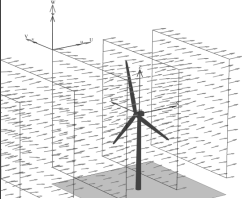
\includegraphics[width=0.7\textwidth]{wind.png}  
            \end{center}
            
            
        \end{column}
    \end{columns}
\end{frame}

% Slide: Actuator Sector Model (ASM) - Concept and Motivation
\begin{frame}{Actuator Sector Model (ASM) - Concept}
    \begin{columns}
        \begin{column}{0.6\textwidth}
                \textcolor{red}{Actuator Line Model Limitations:}
                \begin{itemize}
                \small
                    \item Small time steps required ($\Delta t_F$)
                    \item High computational cost for LES
                \end{itemize}
                
                \textcolor{blue}{Actuator Disk model Advantages:}
                \begin{itemize}
                \small
                    \item Larger time steps possible
                    \item Lower computational cost
                    \item No individual blade information
                \end{itemize}
                
                \textcolor{green!60!black}{Actuator Sector model Solution:}
                \begin{itemize}
                \small
                    \item Detailed blade output + Computational efficiency
                    \item Decoupled time stepping
                \end{itemize}

            
            \textbf{Time Step Decoupling Strategy:}
            \begin{itemize}
            \small
                \item PALM: $\Delta t_P$ determined by CFL/diffusion criteria
                \item FAST: $\Delta t_F < \Delta t_P$ for ALM accuracy
                \item Significant reduction in total computational time
            \end{itemize}
        \end{column}
        
        \begin{column}{0.4\textwidth}
        \begin{center}
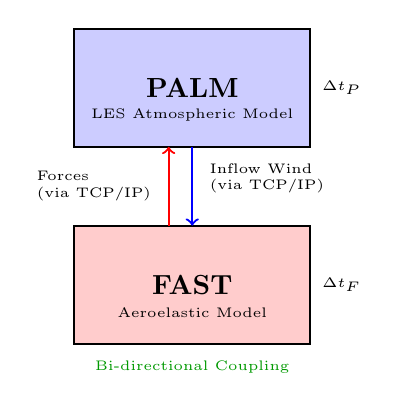
\begin{tikzpicture}
    % PALM box
    \draw[fill=blue!20, thick] (0,3) rectangle (3,4.5);
    \node at (1.5,3.75) {\textbf{PALM}};
    \node[font=\tiny] at (1.5,3.4) {LES Atmospheric Model};
    
    % FAST box
    \draw[fill=red!20, thick] (0,0.5) rectangle (3,2);
    \node at (1.5,1.25) {\textbf{FAST}};
    \node[font=\tiny] at (1.5,0.9) {Aeroelastic Model};
    
    % Arrow from PALM to FAST (Inflow wind)
    \draw[->, thick, blue] (1.5,3) -- (1.5,2);
    \node[font=\tiny, right, align=left] at (1.6,2.6) {Inflow Wind\\(via TCP/IP)};
    
    % Arrow from FAST to PALM (Forces)
    \draw[->, thick, red] (1.2,2) -- (1.2,3);
    \node[font=\tiny, left, align=left] at (1.1,2.5) {Forces\\(via TCP/IP)};
    
    % Time step indicators
    \node[font=\tiny] at (3.4,3.75) {$\Delta t_P$};
    \node[font=\tiny] at (3.4,1.25) {$\Delta t_F$};
    
    % Coupling indication
    \node[font=\tiny, green!60!black] at (1.5,0.2) {Bi-directional Coupling};
\end{tikzpicture} 
        \end{center}

            
            \vspace{0.3cm}
            \small
            ASM allows PALM to use optimal atmospheric time steps while maintaining detailed turbine physics in FAST
        \end{column}
    \end{columns}
\end{frame}

% Slide: ASM Implementation and Technical Details
\begin{frame}{ASM Operational Mechanism}
    \begin{columns}
        \begin{column}{0.6\textwidth}
            \textbf{ASM Operational Steps:}
            \begin{enumerate}
                \item FAST communicates initial blade positions.
                \item PALM provides wind speeds from frozen field
                \item During $\Delta t_P$, rotor sweeps sector: 
                $$\alpha = \Omega \cdot \Delta t_P$$ we take velocities from the central line of the sector 
                \item Using NWC to correct wind speeds
                \item Exchange of current blade positions and velocities
                \item Calculating turbine response.
            \end{enumerate}
            
            \vspace{0.3cm}
            \begin{block}{Technical Benefits}
                \begin{itemize}
                    \item Maintains ALM physics in FAST
                    \item Efficient force projection in PALM
                \end{itemize}
            \end{block}
            %\textbf{Force Distribution (Gaussian Smearing):}
            %$$\eta = \frac{1}{\epsilon^3 \pi^{3/2}} \exp\left(-\frac{r^2}{\epsilon^2}\right)$$
            %where $\epsilon = 2\Delta$ (grid spacing factor)
        \end{column}
        
        \begin{column}{0.4\textwidth}
            \begin{figure}
                \vspace{-1cm}
                \hspace*{-0.7cm} % Move the figure slightly to the left
                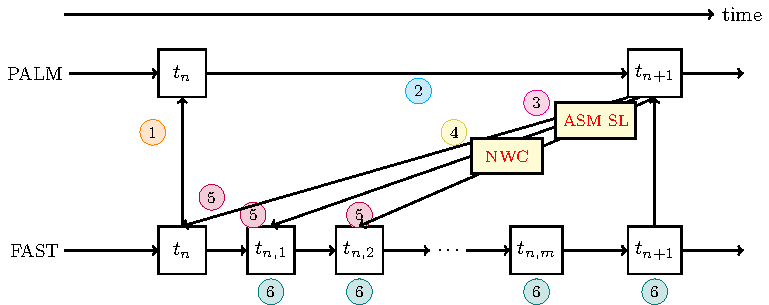
\includegraphics[width=1.2\textwidth]{ASM_representation.pdf}
                \caption{Schematic of the operation mode of the coupling}
                \label{fig:asm_sector}
            \end{figure}
            Based on research work done by \parencite{steinbruck2024, kruger2022}
        \end{column}
    \end{columns}
\end{frame}

% \begin{frame}{ASM Operational Mechanism}
%     \begin{columns}
%         \begin{column}{0.6\textwidth}
%             \textbf{ASM Operational Steps:}
%             \begin{enumerate}
%                 \item FAST communicates initial blade positions.
%                 \item PALM provides wind speeds from frozen field
%                 \item During $\Delta t_P$, rotor sweeps sector: 
%                 $$\alpha = \Omega \cdot \Delta t_P$$ we take velocities from the central line of the sector 
%                 \item Using NWC to correct wind speeds
%                 \item Exchange of current blade positions and velocities
%                 \item Calculating turbine response.
%             \end{enumerate}
%             
%             \vspace{0.3cm}
%             \begin{block}{Technical Benefits}
%                 \begin{itemize}
%                     \item Maintains ALM physics in FAST
%                     \item Efficient force projection in PALM
%                 \end{itemize}
%             \end{block}
%             %\textbf{Force Distribution (Gaussian Smearing):}
%             %$$\eta = \frac{1}{\epsilon^3 \pi^{3/2}} \exp\left(-\frac{r^2}{\epsilon^2}\right)$$
%             %where $\epsilon = 2\Delta$ (grid spacing factor)
%         \end{column}
%         
%         \begin{column}{0.4\textwidth}
%             \begin{figure}
%                 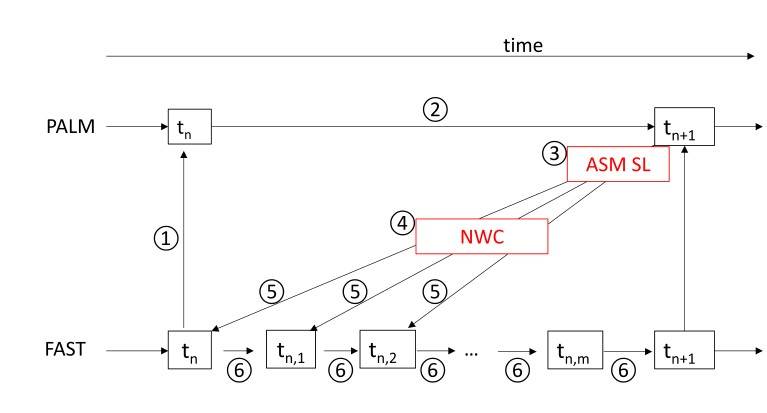
\includegraphics[width=\textwidth]{ASM.jpg}
%                 \caption{Schematic of the operation mode of the coupling}
%                 \label{fig:asm_sector}
%             \end{figure}
%             Based on research work done by \parencite{steinbruck2024, kruger2022}
%         \end{column}
%     \end{columns}
% \end{frame}


\begin{frame}{Force Projection in PALM}

    \begin{columns}[T]
        \begin{column}{0.55\textwidth}
            \textbf{Actuator Sector Method (ASM)}
            \begin{itemize}
            \small
                \item Forces from bold central line applied to all $m$ lines in sector
                \item Gaussian-shaped smearing distributes forces in 3D space
            \end{itemize}
            
            \begin{block}{Gaussian Distribution}
                \begin{equation*}
                    \eta = \frac{1}{\epsilon^3 \pi^{3/2}} \exp\left(-\left(\frac{r}{\epsilon}\right)^2\right)
                \end{equation*}
                where:
                \begin{itemize}
                    \small
                    \item $\eta$ = regularization function
                    \item $r$ = distance from grid node to turbine
                    \item $\epsilon$ = smearing parameter
                \end{itemize}
            \end{block}
            \begin{alertblock}{Key Concept}
                \small
                Forces are not applied as point sources but distributed smoothly using Gaussian smearing to avoid numerical instabilities
            \end{alertblock}
        \end{column}
        
        \begin{column}{0.43\textwidth}
            \begin{figure}
                \centering
                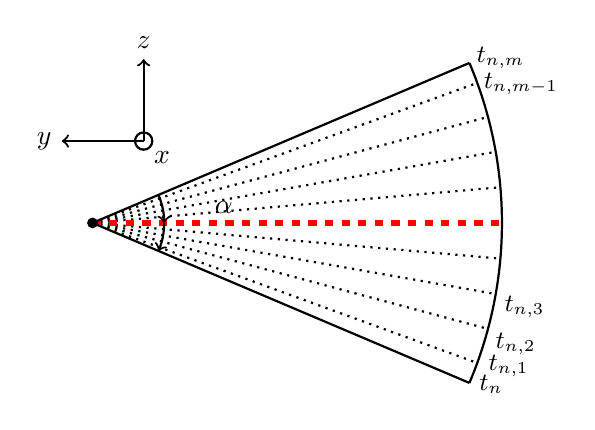
\begin{tikzpicture}[scale=1.3]
                    % Main sector diagram (centered)
                    % Sector parameters
                    \pgfmathsetmacro{\sectorangle}{23}
                    \pgfmathsetmacro{\sectorradius}{4}

                    % Shaded sector (white fill)
                    \fill[white] (0,0) -- (\sectorangle:\sectorradius) 
                        arc (\sectorangle:-\sectorangle:\sectorradius) -- cycle;

                    % Radial lines (m lines) in black
                    \foreach \i in {-4,-3,-2,-1,1,2,3,4} {
                        \pgfmathsetmacro{\lineangle}{\i*5}
                        \draw[dotted, thick, black] (0,0) -- (\lineangle:\sectorradius);
                    }

                    % Central bold line in red
                    \draw[line width=2pt, dashed, red] (0,0) -- (0:\sectorradius);

                    % Sector boundaries in black
                    \draw[thick, black] (0,0) -- (\sectorangle:\sectorradius) node[right,black] {};
                    \draw[thick, black] (0,0) -- (-\sectorangle:\sectorradius) node[right,black] {};
                    \draw[thick, black] (\sectorangle:\sectorradius) arc (\sectorangle:-\sectorangle:\sectorradius);

                    % Labels for some lines (black)
                    \node[text=black] at (22:\sectorradius+0.3) {\small$t_{n,m}$};
                    \node[text=black] at (18:\sectorradius+0.4) {\small$t_{n,m-1}$};
                    \node[text=black] at (-11:\sectorradius+0.3) {\small$t_{n,3}$};
                    \node[text=black] at (-16:\sectorradius+0.3) {\small$t_{n,2}$};
                    \node[text=black] at (-19:\sectorradius+0.3) {\small$t_{n,1}$};
                    \node[text=black] at (-22:\sectorradius+0.2) {\small$t_n$};

                    % Angle alpha covering the entire sector (black)
                    \draw[<-,thick,black] (0:0.7) arc (0:{\sectorangle}:0.7);
                    \draw[->,thick,black] (0:0.7) arc (0:{-\sectorangle}:0.7);
                    \node at (0:1.1) [above right, text=black] {\textbf{$\alpha$}};

                    % Origin point
                    \fill[black] (0,0) circle (1.5pt);

                    % 3D coordinate system at top left in black
                    \begin{scope}[shift={(0.5,0.8)}, scale=0.8]
                        \draw[thick,->,black] (0,0) -- (0,1) node[above] {$z$};
                        \draw[thick,->,black] (0,0) -- (-1,0) node[left] {$y$};
                        \draw[thick,black] (0,0) circle (3pt) node[below right] {$x$};             \end{scope}
                \end{tikzpicture}
                \caption{\scriptsize Sector schematic: values from central line (bold, red) projected to flow. $y$, $z$ = rotor plane; $x$ = streamwise direction}
            \end{figure}
        \end{column}
    \end{columns}

\end{frame}

\begin{frame}{Intended Outcomes}
\begin{tcolorbox}[colback=blue!3!white,colframe=blue!65!black,title=Outcomes:]
\vspace{0.1cm}
    \begin{enumerate}
        \item \textbf{Wake Characterization in Complex Terrain}
        
        \vspace{0.3cm}
        \begin{itemize}
            \item Detailed analysis of wake dynamics over complex terrain
            
            \vspace{0.15cm}
            \item Impact of atmospheric stability on wake evolution
        \end{itemize}
        
        \vspace{0.25cm}
        \item \textbf{Turbine Performance Assessment}
        
        \vspace{0.2cm}
        \begin{itemize}
            \item Power production analysis for downstream turbines
            
            \vspace{0.15cm}
            \item Load variations due to wake interactions
            
            \vspace{0.15cm}
            \item Fatigue damage equivalent loads (DEL) calculations
        \end{itemize}
        
        \vspace{0.25cm}
        \item \textbf{Model Validation}
        
        \vspace{0.2cm}
        \begin{itemize}
            \item Comparison with field measurements (SCADA data)
        \end{itemize}
    \end{enumerate} 
\end{tcolorbox}

\end{frame}
\begin{frame}{Work Done so far:}
\begin{textblock*}{\textwidth}(0cm,1.5cm)
    % Left text
    \begin{minipage}{0.48\textwidth}
        \begin{enumerate}
        \small
            \item Installed and Practiced PALM on Linux and in taifun.
            \item Most of Literature review including selected stull chapters.
            \item Ran ADM-R simulation, rudimentary flow over a hill PALM simulations.
            \item Ran the test simulation of PALM-FAST coupling in taifun.
        \end{enumerate}
    \end{minipage}
    \hfill
    % Right top image
    \begin{minipage}{0.48\textwidth}
        \centering
        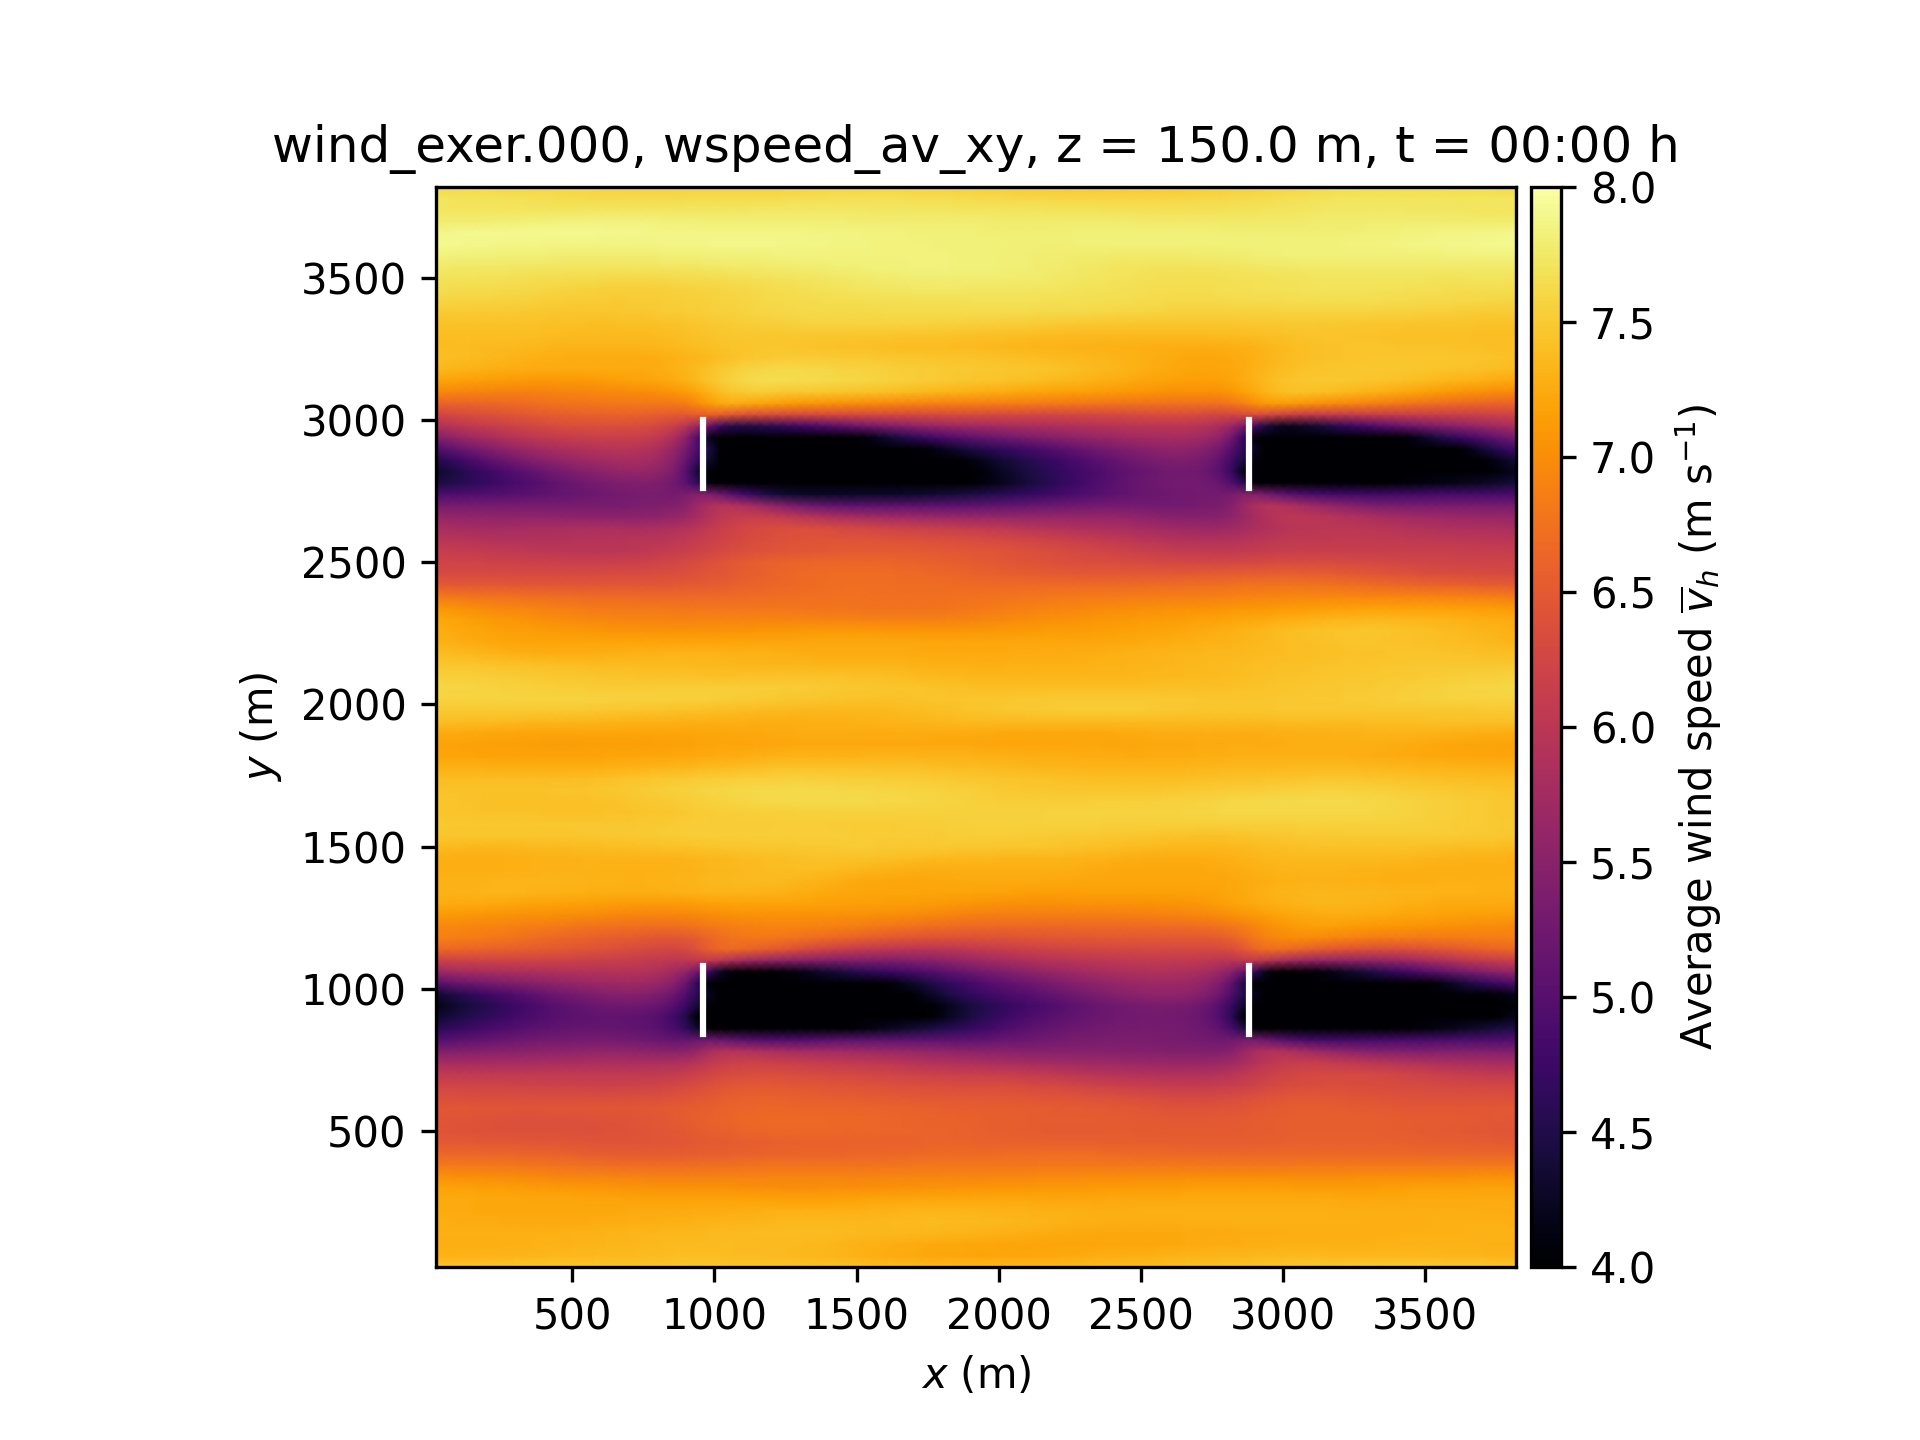
\includegraphics[width=0.8\textwidth]{adr.png}
    \end{minipage}
\end{textblock*}

\begin{textblock*}{\textwidth}(0cm,5.5cm)
    % Bottom left image
    \begin{minipage}{0.48\textwidth}
        \centering
        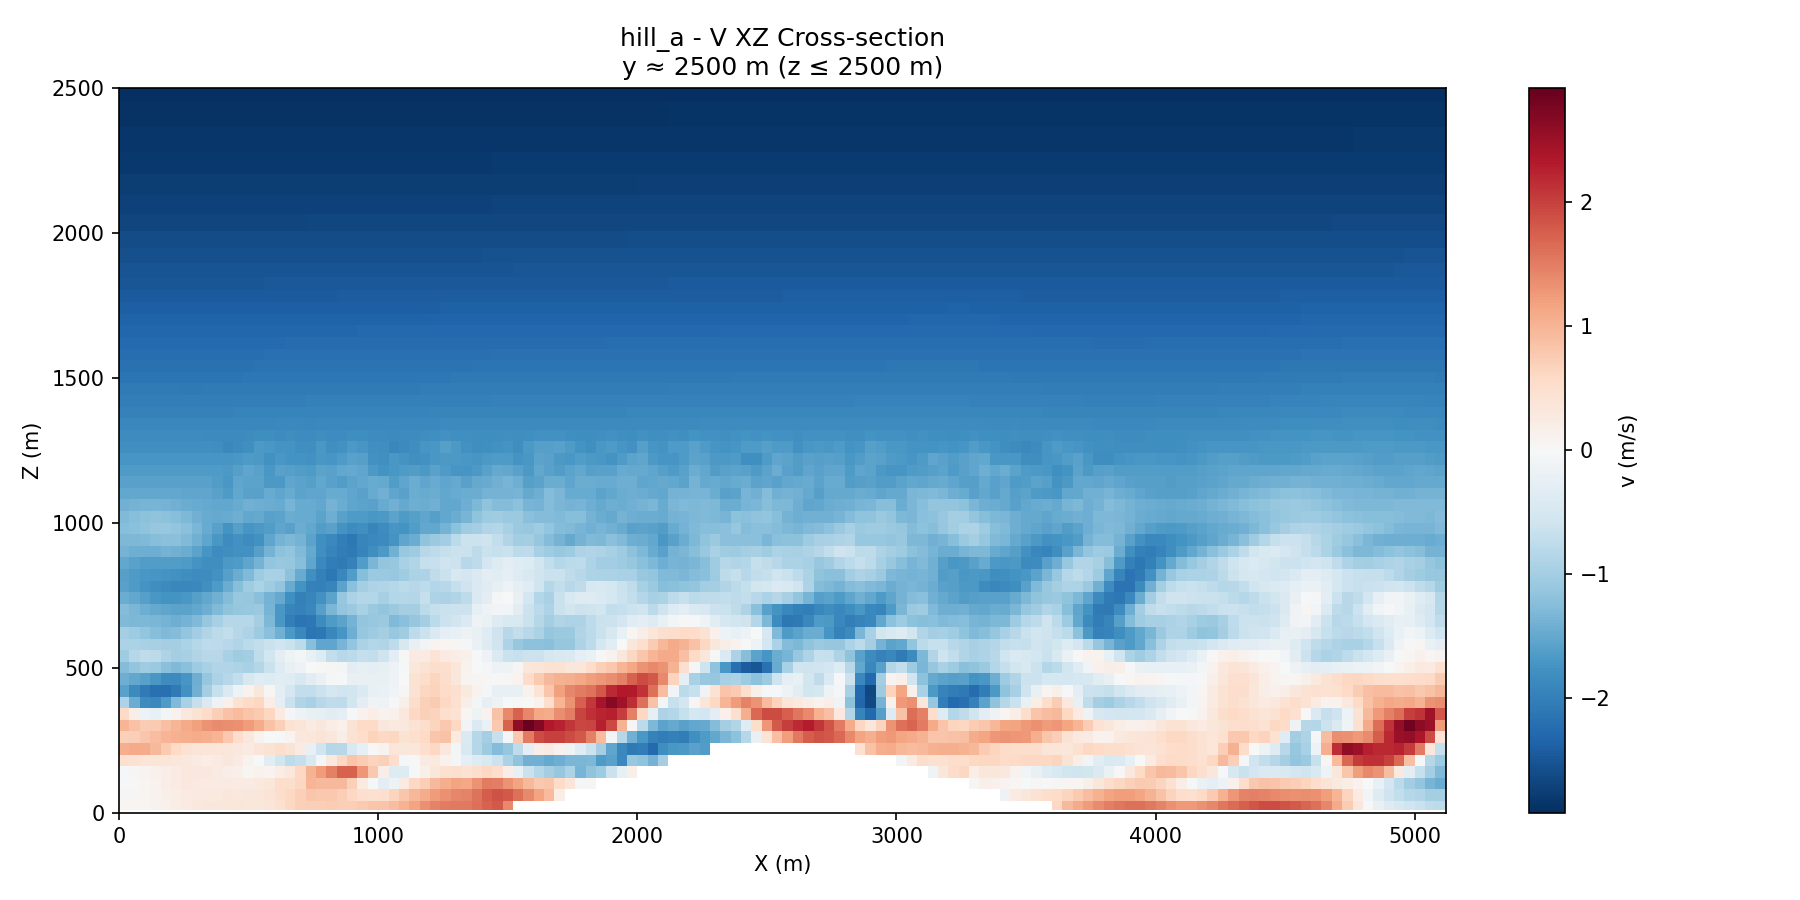
\includegraphics[width=0.9\textwidth]{hill.png}
    \end{minipage}
    \hfill
    % Bottom right image
    \begin{minipage}{0.48\textwidth}
        \hspace{0.5cm} % Move image slightly to the right
        \centering
        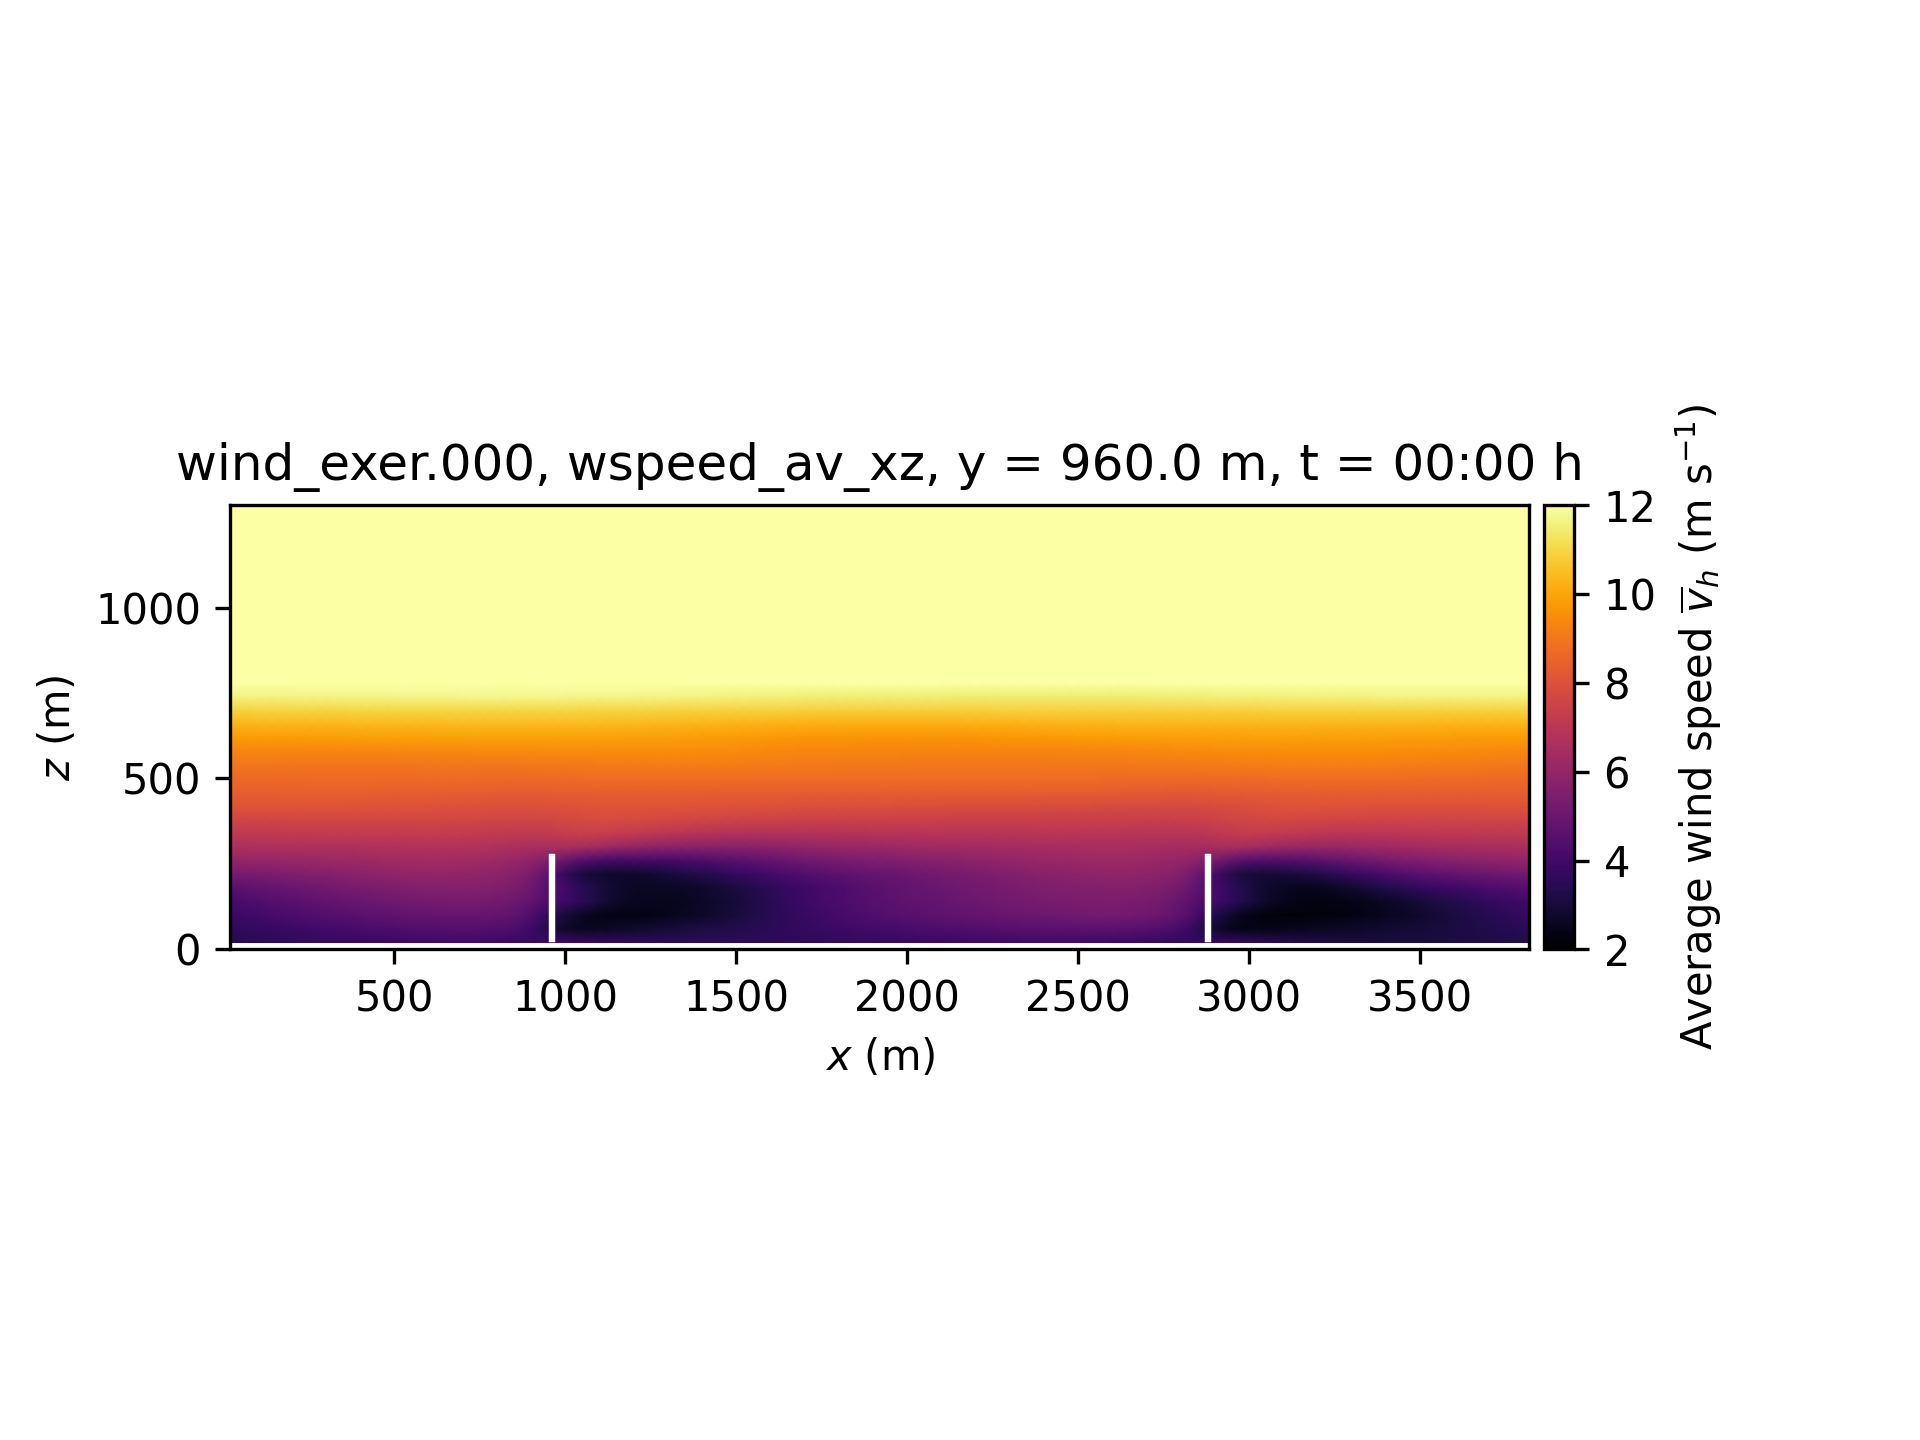
\includegraphics[width=0.9\textwidth]{wtm.png}
    \end{minipage}
\end{textblock*}
\end{frame}
\begin{frame}{References}
    \printbibliography
\end{frame}
\end{document}
